\section{Design}
\label{sec:design}

\subsection{Architecture Overview}
\label{subsec:architecture}

\begin{figure}[t!]
		\centering
		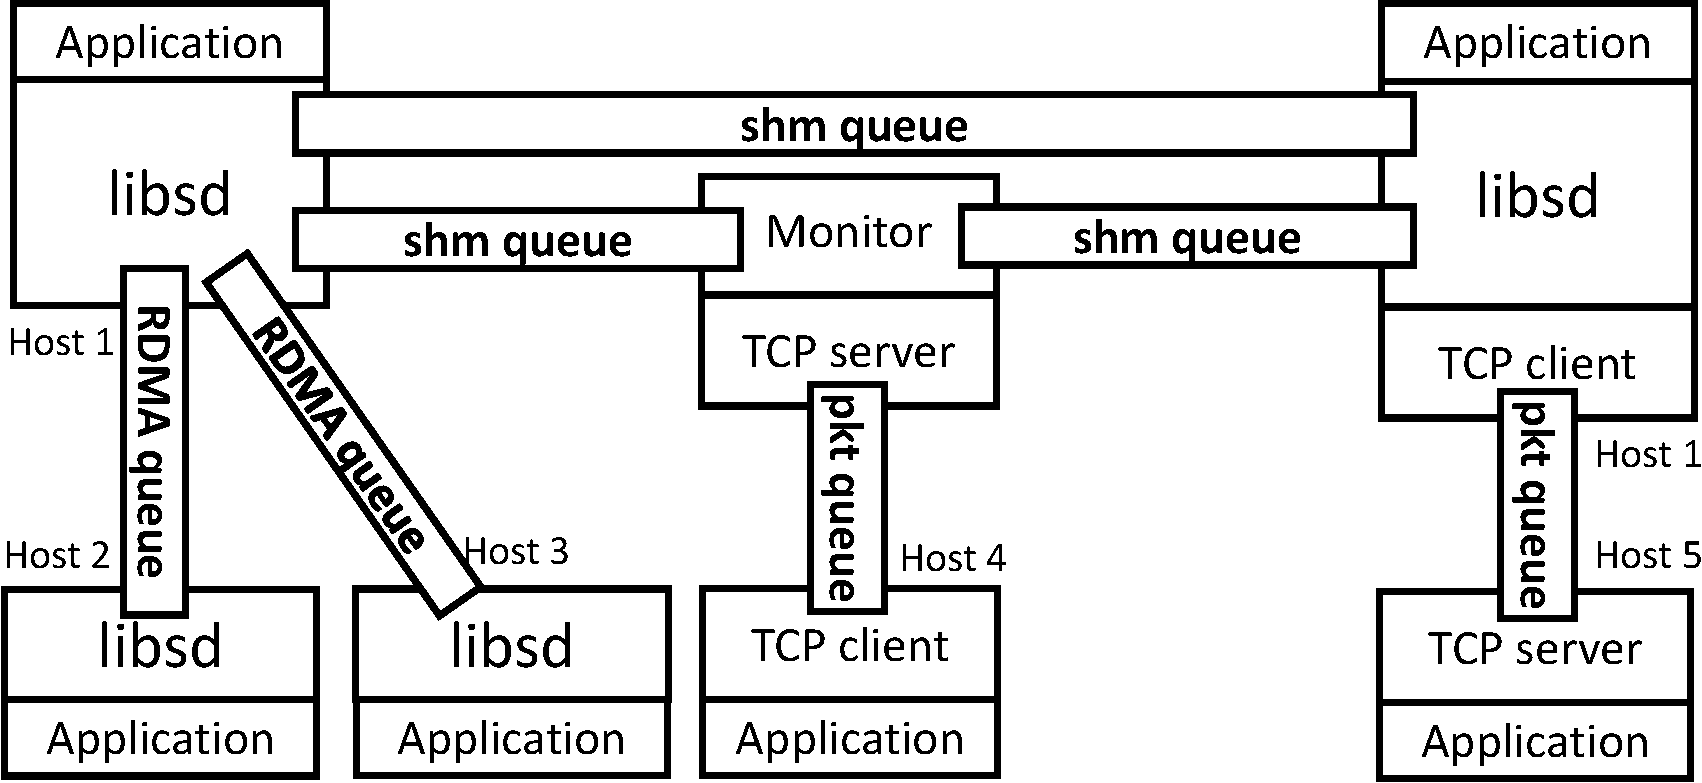
\includegraphics[width=0.49\textwidth]{images/architecture_new}
		\vspace{-15pt}
		\caption{Architecture of \sys{}. Host 1 and 2 are RDMA capable, while host 3 is RDMA incapable.}
		\label{fig:architecture}
		\vspace{-15pt}
\end{figure}


\iffalse
\begin{figure}[t!]
	\centering
	\subfloat[Traditional queue structure.]{
		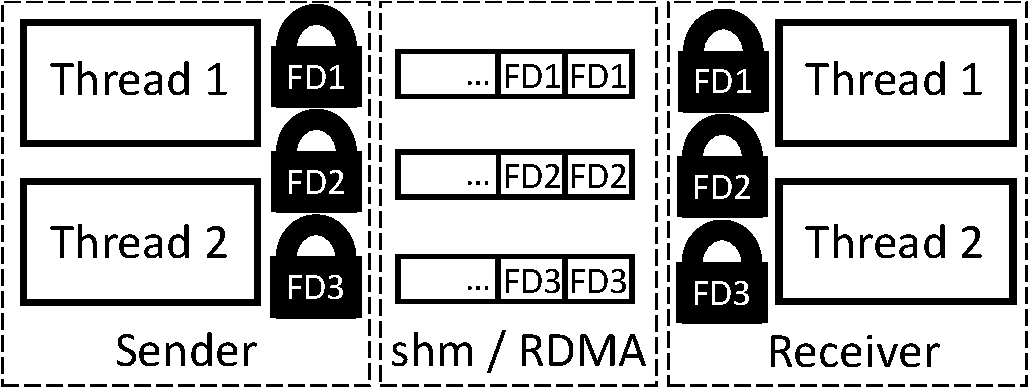
\includegraphics[width=0.4\textwidth]{images/fork_linux}
	}
	\vspace{-5pt}
	\subfloat[\sys{} queue structure.]{
		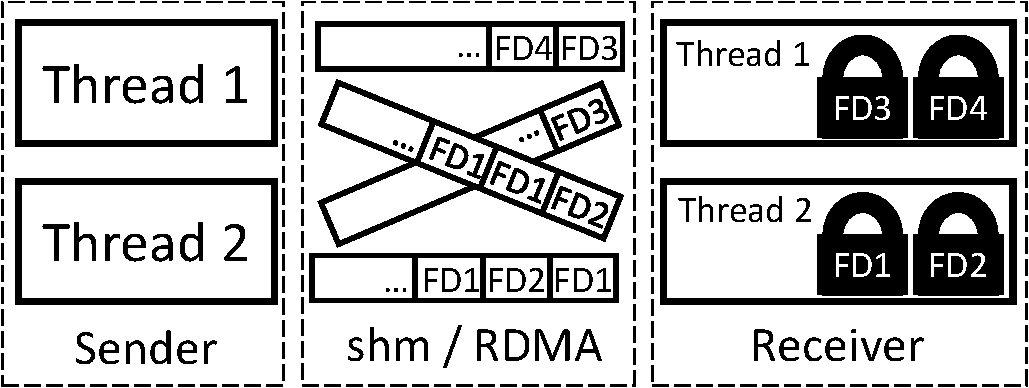
\includegraphics[width=0.4\textwidth]{images/fork_rdwr}
	}
	\vspace{-5pt}
	\caption{Comparison of queue structures. Assume sender and receiver each has two threads. First, \sys{} creates peer-to-peer queues between each pair of sender and receiver threads. Rather than protecting the queue with locks, we designate each FD to a receiver thread to ensure ordering. Second, data from all connections (FDs) are multiplexed through a shared queue, instead of one queue per FD.}
	\label{fig:fork-rdwr}
	\vspace{-10pt}
\end{figure}
\fi


%As shown in Figure~\ref{fig:architecture}, the core component of \sys{} is a user-space library \libipc{}.

Figure~\ref{fig:architecture} gives the architecture of \sys. To use \sys, an application loads a user-space library \libipc{} by setting the \texttt{LD\_PRELOAD} environment variable. \libipc{} intercepts all Linux APIs in \texttt{glibc} that are related to file descriptor operations. It implements socket APIs in user space and forwards the other APIs to the kernel. From a security point of view, because \libipc{} resides in the application address space, we cannot trust its behavior. Therefore, we need a trusted component outside \libipc{} to enforce access control and support overlay networks. 

To this end, we design a \emph{monitor} daemon at each host to coordinate control plane operations, e.g., connection creation. The \emph{monitor} daemon is started at OS initialization time. In each host, all the applications loading \libipc{} must establish a shared memory queue with the host's monitor daemon, forming the control plane. On the data plane, applications build peer-to-peer queues to communicate directly, thus relieving the burden of the monitor daemon.  



%To this end, we regard processes as a shared-nothing distributed system that communicates through message passing.
%We design a secure control-plane protocol between applications and the monitor, and a data-plane protocol between applications.

To achieve low latency and high throughput, \sys{} uses shared memory for intra-host and RDMA for inter-host communication. For intra-host communication, only the local monitor is involved. 
The communication initiator first sends a request to the local monitor, then the monitor establishes a shared memory queue between the two applications (possibly in different containers). Then the two applications can communicate directly.  


%During initialization, \libipc{} connects to the local monitor via a shared memory queue.
%To enforce access control policies and support overlay networks, % and load balance new connections to multiple listeners, 
%connection request is always sent to the local monitor.
%For local peers, the monitor just construct a shared memory queue between the two applications , %so they can communicate directly.

For inter-host communication, the monitors of two hosts are both involved. When an application connects to a remote host, its local monitor establishes a regular TCP connection and detects whether the remote host supports \sys{}.
%When the monitor connects to another host for the first time\RED{Why we need to connect two monitors?}, it establishes a regular TCP connection and detects whether the remote host supports \sys{}.
If so, it establishes an RDMA queue between the two monitors, so that future connections between the two hosts can be created faster. The monitor at the remote side dispatches the connection to the target and helps the two applications establish an RDMA queue, as between host 1 and 2 in Figure~\ref{fig:architecture}. If the remote host does not support \sys{}, it keeps using the TCP connection, as between host 1 and 3 in Figure~\ref{fig:architecture}. The detailed connection management protocol is presented in Sec.~\ref{subsec:connection-management}.

In order to remove synchronization overhead for multi-threaded applications, we treat each thread as a separate process.
%Although threads in a process share memory, we use thread-specific storage for most states in \libipc{}.
For two communicating applications, we create peer-to-peer queues between each pair of sender and receiver threads to avoid synchronization cost of contending on the same queue.
In Sec.~\ref{subsec:fork}, we present the peer-to-peer queue design that preserves FIFO ordering semantics and avoids starvation, especially when a process forks or creates a new thread.
To maintain performance with many concurrent connections, rather than creating separate queues for each connection, we multiplex data from all connections through one queue.
In Sec.~\ref{subsec:multiplex-conn}, we present the design of multiplexed queue that avoids head-of-line blocking and supports fetching data from any multiplexed connections.

%Inspired by Unikernels~\cite{madhavapeddy2013unikernels}, we move networking and IPC functions from the kernel to user space. Similar to existing works~\cite{peter2016arrakis,jeong2014mtcp,libvma}, we leverage multiple queues in modern NICs to enable user-space direct access to network. %The kernel is still responsible for process creation, scheduling, virtual memory and device management, but no longer on the critical path of performance.
%To maintain compatibility with existing Linux applications, we design a user-mode library \libipc as a drop-in replacement of the system call wrappers in the GNU C library (glibc). \libipc{} implements network socket functions in user mode, and adds a wrapper to other system calls to track process creation and memory allocation. \libipc{} is not considered a secure domain, as it shares memory space with the application. When \libipc{} is loaded, it creates a Linux native \textit{bootstrap socket} to the \textit{monitor} daemon, then creates a shared memory queue to the monitor.

%Even though multiple threads in the same process share memory space, we still treat each thread as a separated process and use thread-specific storage to store states in \libipc. In the following text, unless explicitly mentioned, we use a ``process'' to refer to a regular process or a thread.




\subsection{Connection Management}
\label{subsec:connection-management}

Before designing the connection management protocol, we keep the following requirements in mind:
1) The applications and \libipc{} are not trusted because they are in the same memory address space. We must enforce access control policies outside \libipc{} to prevent access to restricted resources.
2) Each address and port may be listened by multiple processes, which needs load balancing while avoid starvation.
3) The applications may be in an overlay network and thus needs address translation. 
%4) Multiple concurrent connections may be created between two hosts and therefore should be accelerated.
4) A client should be able to connect to \sys{} and regular TCP/IP hosts transparently, and a server should accept connections from all hosts.

These design requirements lead to a \emph{monitor} service running as a daemon process in each host.
Rather than delegating all operations to the monitor, we only delegate connection creation, which forms the control plane.
From the application's perspective, connection creation is similar to TCP handshake.
Monitor(s) on the path between client and server applications proxy the handshake commands and help them establish a peer-to-peer queue via shared memory or RDMA.
If the remote peer does not support \sys{}, all future operations with it will be delegated to the local monitor.
The detailed procedure is as follows.


\parab{Initialization.}
During initialization, \libipc{} connects to the monitor in local host via \emph{bootstrap socket} (a Unix domain socket or kernel TCP socket on localhost or overlay network) and establishes a shared memory queue between them.
After that, communication between the application and monitor goes through the shared memory queue.

\parab{Socket creation.}
An application first creates a socket identified by an integer \emph{file descriptor} (FD).
Socket FDs and other FDs (e.g. disk files) share a namespace and Linux always allocates the lowest available FD.
To preserve this semantics without allocating dummy FDs in the kernel, \libipc{} intercepts all FD-related Linux APIs and maintains a FD translation table to map each application FD to a user-space socket FD or a kernel FD.
When an FD is closed, \libipc{} put it to a \emph{FD recycle pool}.
Upon FD allocation, \libipc{} first tries to obtain an FD from the recycle pool.
If the pool is empty, it allocates a new FD by incrementing a \emph{FD allocation counter}.
The FD recycle pool and allocation counter are shared among all threads in a process.% and allow wait-free access with atomic operations.

\parab{Bind.}
After socket creation, the application calls \texttt{bind} to allocate address and port.
Because addresses and ports are global resources with permission protection, the allocation is coordinated by the monitor.
As shown in Figure~\ref{fig:conn-setup}, \libipc{} sends the request to monitor and the monitor sets up an address translation rule between physical and overlay network.
\libipc{} employs an optimization to return success speculatively if the bind request would not fail, e.g., when port is not specified for client-side sockets.

\parab{Listen.}
When a server application is ready to accept connections from clients, it calls \texttt{listen} and notifies the monitor.
The monitor maintains a list of listening processes on each address and port to dispatch new connections.
The monitor also uses a user-space networking stack (modified LibVMA~\cite{libvma} in our implementation) or \texttt{netfilter} to wait for incoming TCP SYN packets.
To avoid the kernel networking stack from receiving SYN, the monitor inserts flow steering rules in modern NICs or \texttt{iptables} filters.

\parab{Connect.}
A client application calls \texttt{connect} and sends a SYN command to monitor via shared memory queue.
The monitor translates IP addresses and ports for overlay network, then forwards the SYN to the target server application.
If it is in the same host, forward the SYN to it directly.

\parab{Differentiate \sys{} peers from regular TCP/IP peers.}
If the target is in a different host, the monitor first needs to detect whether the host supports \sys{}.
To this end, the monitor sends a TCP SYN packet with a special option over the network.
If the host is \sys{} capable, its monitor would receive the special SYN and knows the client is \sys{} capable.
The server then responds SYN+ACK with special option, including credentials to setup an RDMA connection, so that the two monitors can communicate through RDMA afterwards.
If either the client or the server monitor finds out that the peer is a regular TCP/IP host, it notifies the application to delegate future operations to itself, 
then executes delegated socket operations via the user-space TCP stack, as shown between host 1 and 3 in Figure~\ref{fig:architecture}.

\parab{Dispatch new connections to listeners.}
Let's continue with the connect creation procedure assuming that both ends support \sys{}.
In Linux, new connection requests are queued in a \emph{backlog} in the kernel.
Every time the server calls \texttt{accept}, it accesses the kernel to dequeue from the backlog, which requires synchronization and adds latency.
In contrast, we maintain a per-listener backlog for every thread that listens on the socket.
The server monitor distributes SYN to a listener thread in round-robin manner.

Dispatching connection to listeners may lead to starvation when a listener does not \texttt{accept} new connections.
We devise a \textit{work stealing} approach.
When a listener invokes \texttt{accept} while the backlog is empty, it requests the monitor to steal from others' backlog.
%To avoid polling empty backlogs, each listener notifies the monitor when its backlog becomes empty.
To avoid contention between a listener and monitor, the monitor sends a request to the listener to steal from the backlog.

\parab{Establish a peer-to-peer queue.}
The first time a client and a server application communicates, the server monitor helps them establish a direct connection.
For intra-host, the monitor allocates a shared memory queue and sends the shared memory key to both client and server applications.
For inter-host, the client and server monitors establish a new RDMA QP, and send the local and remote keys to the corresponding applications.
To reduce latency, the peer-to-peer queue is established by monitor(s) when the SYN command is distributed into a listener's backlog.
However, if the SYN is stolen by another listener, a new queue needs to be established between client and the new listener, as shown in the Wait-Server state of Figure~\ref{fig:conn-setup}.

\parab{Finalize connection creation.}
After the server sets up peer-to-peer queue, as the left side of Figure~\ref{fig:conn-setup} shows, the server application sends a ACK to client application containing the client FD in SYN request and its allocated server FD.
Similar to TCP handshake, the server application can send data to the queue after sending the ACK.
When the client application receives the ACK, as shown on the right side of Figure~\ref{fig:conn-setup}, it sets up the FD mapping and can start sending data.

\begin{figure}[t!]
	\centering
	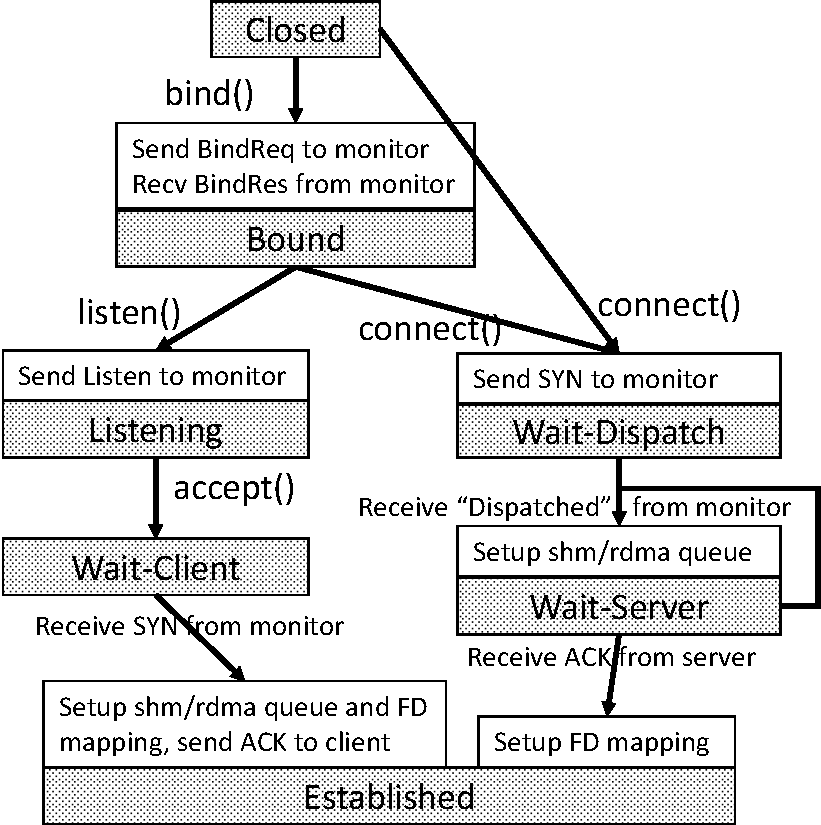
\includegraphics[width=0.3\textwidth]{images/conn-setup-new}
	\vspace{-5pt}
	\caption{State machine of connection creation in \libipc{}.}
	\vspace{-10pt}
	\label{fig:conn-setup}
\end{figure}
\begin{figure}[t!]
	\centering
	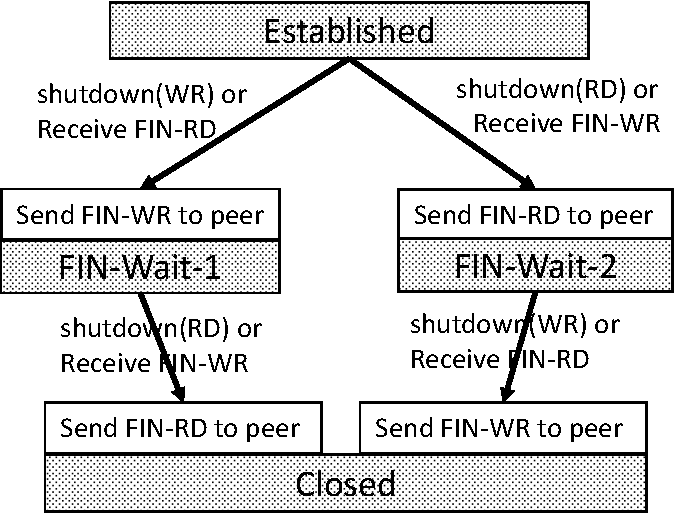
\includegraphics[width=0.25\textwidth]{images/conn-close-new}
	\vspace{-5pt}
	\caption{State machine of connection close in \libipc{}.}
	\label{fig:conn-close}
	\vspace{-15pt}
\end{figure}


\parab{Connection close.}
Closing a connection is fully peer-to-peer and does not need to involve the monitor.
Because both shared memory and RDMA are reliable and ordered communication channels, the connection close procedure is simpler than TCP.
However, we still require a handshake between peers before the FD is deleted and possibly reused by a new connection.
Otherwise, the peer might not yet have received the close message, thus sends data to the wrong connection.
Because socket is bidirectional, \texttt{close} is equivalent to \texttt{shutdown} on both send and receive directions.
As Figure~\ref{fig:conn-close} shows, when application shuts down one direction of a connection, it sends a \emph{shutdown message} to the peer.
The peer responds with a shutdown message.
A process deletes an FD when it receives shutdown messages in both directions.



\iffalse

\parab{\texttt{Bind} and \texttt{listen}.}
A \emph{server} process \texttt{bind}s a socket and needs to detect IP and port conflict. In this case, \texttt{bind} is non-partitionable and goes to the monitor. The monitor also listens on the IP and port in a user-space TCP/IP stack (\textit{e.g.} mTCP~\cite{jeong2014mtcp}, LibVMA~\cite{libvma} or Seastar~\cite{seastar}) to receive connections from other hosts.

A \emph{client} process typically \texttt{bind}s without specifying IP and port, so we need to allocate a unique IP and port for it. For scalability, we partition the loopback IP address space (127.0.0.0/8) and each process allocates IP and port in its range.

\parab{\texttt{Connect} and \texttt{accept}.}
When a client process connects to a server process on the same host, it sends a \textit{connect request} to the monitor via shared memory queue. When the server process is on another host, it creates a \textit{bootstrap TCP socket} with a special option via the user-space TCP/IP stack. If the server host supports the option, it is a \sys host and its monitor establishes an RDMA connection to the client to speedup later communications. Otherwise, the client process keeps using the bootstrap TCP socket for compatibility.

On a server host, the monitor distributes connect requests to server processes in a round-robin order, and a \textit{backlog} is maintained in each process. If the client is TCP only, the monitor proxies messages between the server process and the user-space TCP/IP stack. If the client is intra-server or RDMA capable, and it is the first time for the client and server processes to communicate, the monitor creates an inter-process queue for the process pair and sends the credentials to both processes via bootstrap sockets. After a server process \texttt{accept}s a connection in the backlog, it sends a message to the client via inter-process queue to create an FD mapping, then the socket is ready for data transmission. As Figure~\ref{fig:conn-setup} shows, connection creation takes three inter-process delays.

Distributing connection to listeners may lead to starvation when a listener does not \texttt{accept} new connections. We devise a \textit{work stealing} approach. When a listener \texttt{accept}s from empty backlog, it requests the monitor to steal from others' backlog. To avoid polling empty backlogs, each listener notifies the monitor when its backlog becomes empty. To avoid contention between a listener and monitor, the monitor sends a request to the listener rather than stealing from the backlog directly.

%\subsubsection{Connection Close}

\parab{\texttt{Close} and \texttt{shutdown}.}
Connection close is a peer-to-peer operation because only the peer process needs to be notified. If FD is deleted immediately after \texttt{close}, a new connection may reuse the FD while the peer process might not yet have received the close event thus sends data to the wrong connection. To avoid this, we require a handshake between peers.
Because socket is bidirectional, \texttt{close} is equivalent to \texttt{shutdown} on both send and receive directions.
When application shuts down one direction of a connection, it sends a \textit{shutdown message} to the peer. The peer responds with a shutdown message. A process deletes an FD when it receives shutdown messages in both directions.

%In order to achieve high scalability, we separate scalable operations to different processes. To avoid the overhead of contention, \libipc enable the file descriptor allocation by individual process and when a connection is setup, the other peer of the connection gets notified of the file descriptor number by message passing. Since we treat different threads in one process as different processes, we allocate file descriptor of different ranges to each of them to avoid collision. Since file descriptor is managed separately by each process, it is possible that a file descriptor is reused after the connection is closed. Our solution is that resources of a file descriptor is not released until an ACK is received for the close operation.

%Generally, each process in our design is treated as an endpoint in the network. Figure \ref{fig:conn-setup-close} shows the process of connection setup and close. When \textit{socket} is called, the process itself allocate per fd resources. When \textit{listen} is called, monitor is notified of port occupation. During the \textit{connect} operation, monitor first chooses one of the processes listen on this port then coordinates the creation of the shared memory between the two processes and notifies each other of the new connection. When \textit{close} happens, both of the endpoint notify each other and monitor is responsible to destroy the shared memory between them. 

\fi




\subsection{Sharing a Socket Among Processes}
\label{subsec:fork}

Socket sharing among processes and threads are ubiquitous in modern applications.
Our aim is to maximize the common-case performance while preserving the FIFO semantics.
We make two observations: First, fork and thread creation are infrequent in high performance applications. 
Second, it is uncommon that several processes receive concurrently from a shared socket, because the byte-stream semantics of socket makes it hard to avoid receiving partial messages.
%For such producer-consumer scenarios, message brokers~\cite{hintjens2013zeromq,rabbitmq2017rabbitmq,kreps2011kafka} are typically used.
Based on the observations, we propose the following requirements:

\begin{enumerate}[noitemsep,nolistsep]
 \item \textbf{Synchronization-free.} With multiple senders and receivers, if only one pair of sender and receiver is active, no synchronization should occur.
 \item \textbf{Multi-sender scalability.} Multiple processes may send data concurrently through a shared socket. With multiple active senders and a single receiver, if the receiver is not a bottleneck, the throughput should scale.
 \item \textbf{Self-stabilization.} Certain operations (\textit{e.g.} \texttt{fork}) may slow down the system temporarily, but after that the performance should converge back to normal.
\end{enumerate}

For compatibility with Linux semantics, we also need to ensure message ordering and liveness:
\begin{enumerate}[noitemsep,nolistsep]
\item \textbf{Single receiver ordering.} For a specific pair of sender and receiver, the received messages have the same ordering as they were sent.
\item \textbf{Multiple receiver ordering.} The order of \texttt{send} and \texttt{recv} operations for one sender and multiple receivers should be linearizable. If receiver $R_1$ receives $D_1$ before receiver $R_2$ calls \texttt{recv} and gets $D_2$, we guarantee that $D_1$ is sent before $D_2$.
\item \textbf{Deadlock-free.} If a socket buffer is not empty when \texttt{recv} is called by one or more receivers, at least one receiver should get data.
\item \textbf{Starvation-free.} If a sender keeps sending, any receiver trying to \texttt{recv} will eventually get some data.
\end{enumerate}

We present our scalable socket design in four parts: a) data transmission (\texttt{send} and \texttt{recv}), b) adding new senders and receivers (\texttt{fork} and thread creation), c) connection creation and d) connection close.

\subsubsection{Send/Recv Operation}
\label{subsubsec:fork_rdwr}

In this section, we assume that a socket is connected and the number of senders and receivers are constant.

\parab{Multiple concurrent senders.}
In order to avoid synchronization, we create queues between \emph{every} pair of senders and receivers. %The queues form a bipartite graph between senders and receivers. 
Each receiver polls messages from all sender queues in round-robin order. Therefore, the multi-sender throughput can scale.
%Figure \ref{fig:fork-bipartitegraph} shows a sample of the shared-memory buffers between senders and receivers for one connection.

\parab{One exclusive receiver.}
Each sender, though has a queue to every receiver, designates only a single receiver with exclusive access to the socket and only send data through the corresponding queue.
For example, R1 is designated by both senders in Figure~\ref{fig:fork-p2p}.
In the common cases with only a single active receiver, the performance would be the same as one-to-one communication. 
%It is challenging for the sender to choose a receiver, since the chosen one may not call \texttt{recv}, while other receivers may be under starvation. 

\parab{Switch to a receiver.}
When a non-designated receiver attempts to \texttt{recv} from the socket, it sends a \textit{takeover request} to the sender. 
Up receiving the request, the sender %processes takeover requests in FIFO order to avoid starvation and 
designate the requester as the new exclusive receiver and remove the status from the old designated receiver.
%Another challenge is that when a receiver should send a takeover request. 
%Each receiver maintains a flag locally to indicate whether it is designated by the sender. The flag is flipped when the receiver gets takeover request or completion from sender. When a receiver tries to \texttt{recv} and finds itself not designated, it sends a takeover request to sender. Before the receiver becomes designated, the takeover request is sent only once.

\parab{Remaining data in queue.}
A challenge arise when there is remaining data in the queue when a receiver requests to take over the socket. %We need to ensure that all the remaining data can be received by the new receiver. 
%Because multiple sockets share a queue from sender to each receiver, and different sockets have different designated receivers, the new receiver cannot access the queue from the old receiver directly. Instead, 
The remaining data needs to migrate from the old active queue to the new active queue. When the sender processes a takeover request, it first forwards it to the current receiver. Upon receiving takeover request, the current receiver returns all remaining data to sender via \textit{takeover completion} messages, which the sender forwards to the new receiver. During migration, the sender blocks \texttt{send} operations and takeover requests to ensure message ordering.



%\begin{figure}[t]
%	\centering
%	
\includegraphics[width=0.3\textwidth]{images/fixme}
%	\caption{This figure shows a stable connection handled by multiple senders and receivers.}
%	\label{fig:fork-bipartitegraph}
%\end{figure}

\subsubsection{Fork and Thread Creation}
\label{subsubsec:fork_fork}


\begin{figure}[t]
	\centering
	\subfloat[Traditional locking]{
		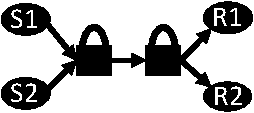
\includegraphics[width=0.15\textwidth]{images/one_conn3}
		\label{fig:fork-locking}
	}
	\hspace{0.02\textwidth}
	\subfloat[SocksDirect peer-to-peer]{
		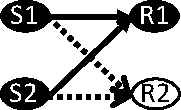
\includegraphics[width=0.11\textwidth]{images/one_conn1}
		\label{fig:fork-p2p}
	}
	\hspace{0.02\textwidth}
	\subfloat[S2 forks to S2' and S3]{
		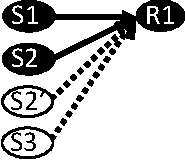
\includegraphics[width=0.1\textwidth]{images/one_conn2}
		\label{fig:fork-fork}
	}
	\vspace{-10pt}
	\caption{Inter-process queue architectures for a shared socket. Dashed arrows represent non-activated queues.}
	\vspace{-15pt}
\end{figure}


%The first challenge with fork and thread creation is how to identify and isolate parent and child processes. 
To identify and isolate parent and child processes, when an application calls \texttt{fork}, \texttt{clone} or \texttt{pthread\_create}, \libipc{} first generates a secret for pairing, then invokes the corresponding system call. After fork, parent and child independently creates a shared memory queue to the monitor and sends the secret (child inherits parent memory space and knows the secret). The monitor can thus pairs the child process with the parent. 
To maintain isolation between parent and child, monitor creates new shared memory queues to replace all queues in \emph{both} parent and child, as Figure~\ref{fig:fork-fork} shows. We do not reuse queues due to potential isolation violation. %The monitor then sends credentials of new queues to parent and child via bootstrap sockets. 
Each peer process is notified of the new queues and the new process. From then on, parent and child processes have isolated queues to the monitor and peers.

%A harder challenge comes from socket connection sharing between parent and child processes. 
Upon fork, each connection needs to add a sender to the sending direction and a receiver to the receiving direction. A major challenge is how to handle the remaining data in the original send and receive queues.

%For each unidirectional queue, we discuss the behavior of related processes in four cases:
%\begin{enumerate}
%	\item A sender process itself forks.
%	\item A receiver of a sender process forks.
%	\item A receiver process itself forks.
%	\item A sender of a receiver process forks.
%\end{enumerate}

%The general process of fork is that after monitor is notified of the fork, it creates shared memory between the newly created process and all the processes which previously have connections with the parent process. The key challenge lies in the fork is that how to deal with the existing data in the connection to guarantee the order requirements.

\parab{Receiver fork.}
First we look at a simple case when a receiver forks. Recall that only one receiver has exclusive access to a socket, as stated in Sec.~\ref{subsubsec:fork_rdwr}. The parent process inherits receive permission. When a sender receives fork notification of its peer, it copies all data from original queues to new queues of the parent process.

\parab{Sender fork.}
When a sender forks, things are more complicated. We need to guarantee that all data sent prior to \texttt{fork} is consumed before the data sent after \texttt{fork}.

Our solution is to let receivers drain the original queue first before switching to the new queues. After \texttt{fork}, both parent and child send data to its new queue. When the receiver is notified of the fork, it keeps track of the original queue and consumes all data in it before activating new queues. Note that the parent or child may fork again before the original queue is drained. With this in mind, the receiver maintains a forest data structure to track dependency of queues. The root of each tree in the forest is the oldest queue to receive from. Each non-leaf node has two children indicating the new queue of parent and child processes. If a non-leaf root queue becomes empty, it will be removed, and the two children queues will be promoted to root nodes.

\parab{Takeover During Fork.}
After a sender forks, the receivers still need the takeover mechanism to arbitrate remaining messages in the original queue. However, both parent and child senders have dropped the original queue and will not respond to takeover requests. A similar situation occurs when a sender process dies. Our solution is to let the receivers use atomic operations to compete for remaining data in the original queue. Since this case rarely happens, the performance of the overall design is not affected.


%Things become much more complicated when cases 1,4 happens after cases 2,3 happening. After receiver forks, the unique sender is responsible for receiving ``takeover message'' and resend the data to new receivers. However, if sender forks following the receiver forks, according to the methods we mentioned above, there is no sender responsible for processing ``takeover message''. Our solution is that we require the receivers to poll the data from the old shared memory queue and compete for data. Since this case rarely happens, the performance of the overall design is not affected.

\subsubsection{Connection Creation}
\label{subsubsec:fork_new}

A connection created by a thread can be accessed by all threads in the same process.
To avoid creating redundant queues and connection states, \libipc does not share the FD eagerly with other threads, because most threads in existing applications do not use connections created by other threads.
When a thread do want to accesses a FD that belongs to another thread, \libipc sends a message to the owner thread and requests sharing the FD. %This procedure is exactly the same as sharing existing connections during thread creation (Sec.~\ref{subsubsec:fork_fork}). %The sharing procedure only happens once for every connection and thread. Sharing existing connections eagerly during thread creation is an optimization. First, children threads are more likely to use existing connections than siblings. Second, batch processing improves performance.

\subsubsection{Connection Close}
\label{subsubsec:fork_close}

%Close is the operation that all of the processes leave the connection. The synchronization is  especially challenging since all the processes are run in parallel. One challenge lies in file descriptors are managed by decentralized processes and are possibly reused. One process close a connection while the others are doing compute intensive tasks is a case. It is possible that the file descriptor of the old process is reused and a new connection is setup with the same file descriptor. The other process may notice the close of the old connection and also call close on its own side, which lead to the new connection setup by the previous process closed due to the match of same file descriptor. 

%To satisfy the synchronization requirements, the close function call is all completed by message passing. The caller of close need to wait for ACK from all the other peers before release resources. i.e. the status of the connection.

%\parab{Broadcast.}
%When a process calls \texttt{close}, all its peers cannot send to or receive from the FD. In this sense, 
Closing a shared connection needs to multicast a notification to the peers and collect responses from them. A challenge arise when \texttt{close} is interleaved with \texttt{fork}. Since \texttt{fork} and \texttt{close} do not commute~\cite{clements2015scalable}, we need a rule to determine their partial order. We make the choice that the ordering is determined by the initiator of \texttt{close}. If a process calls \texttt{close} before receiving fork notification, it will piggyback close notification with fork completion to both parent and child processes.

%\parab{Handshake before releasing resource.}
%Another challenge is caused by FD reuse after close. As stated in Sec.~\ref{subsec:socket-api}, a FD is deleted after receiving shutdown message of both directions. With multiple processes sharing a connection, after one process calls \texttt{close}, others can still use the connection. Consequently, a process deletes a FD only after receiving shutdown messages of both directions from all peers of the FD.

%Another challenge lies in the close of a connection is that close is a broadcast operation while send/receive is sent to a specific process. Besides, fork and close are immutable operations while the scalability requirements of the system impose the constraint that all the operations run asynchronously. As a result, a rule to determine the partial order is required.

%In \libipc, we make the choice that the order of fork and close is determined at the start point of the fork operation and the end point (after receiving all the ACKs). By making this choice, when a process waiting fork close ACK encounters fork message, it could send a separate close request to newly created process, which guarantees all the processes closed.


\subsection{Multiplex Sockets via One Queue}
\label{subsec:multiplex-conn}

\begin{figure}[t]
	\centering
	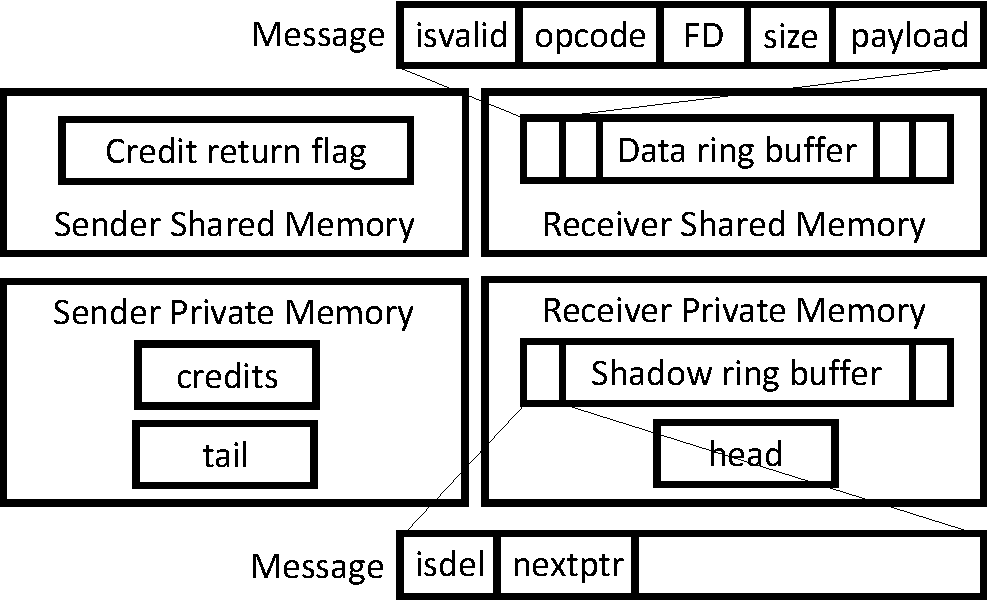
\includegraphics[width=0.4\textwidth]{images/locklessq_new}
	\vspace{-5pt}
	\caption{The structure of an inter-thread queue.}
	\vspace{-15pt}
	\label{fig:locklessq-structure}
\end{figure}


%\parab{Multiplex connections in event-driven applications.}
To reduce memory footprint and improve locality of memory accesses, we use one queue to multiplex all connections between a pair of threads. Each data item in the queue is marked with its FD. By using a single queue, we reduce per-socket memory footprint, random memory accesses and cache misses.

\parab{Message format.}
As shown in Figure~\ref{fig:locklessq-structure}, the main component of the queue is a \emph{data ring buffer}, where messages are stored back-to-back.
Each message in the ring buffer consists of an 8-byte header and a variably sized payload. The header consists of an \textit{isvalid} flag, an opcode, the receiver's FD number and the payload size. Messages are aligned to 8 bytes to ensure header write atomicity.% and accelerate payload copy.

\parab{Event polling.}
We maintain a bitmap of each epoll FD set.
When \texttt{epoll\_wait} is called, we scan all data queues round-robin and check the FD of each data message against the bitmap. If the FD is in the bitmap, an event is returned to the application.
A global cursor exists to resume data queue scanning from the last position in the last scanned queue.

A per-queue cursor records the last scanned position in each queue to avoid scanning a message multiple times.
To speedup repeated receive operations of a specific FD, we build a linked list of messages for each FD as a side product of event polling.
Each FD maintains positions of the first and last scanned but unread messages of the FD.
When a new message of the FD is scanned, the \emph{nextptr} pointer in the last message is updated to point to the new message.

To poll events from sockets and other FDs (handled by kernel) at the same time, \libipc{} creates an \textit{epoll thread} in each process to wait on all FDs handled by kernel. When it receives a kernel event, it broadcasts the event to application threads via shared memory queues. %\texttt{Epoll\_wait} in \libipc{} will return such kernel events in addition to socket events. %Note that Linux allows an event to be received by multiple threads sharing the FD.

\parab{Pick from middle of queue.}
In order to support receiving data from a specific FD, the queue needs to support picking a message in the middle with a specific FD.
Fortunately, this does not happen frequently. Event-driven applications typically process incoming events in a FIFO order. For \texttt{epoll\_wait} in level trigger mode, we iterate through all messages in the queue and return those in the set of registered FDs. When applications call \texttt{recv}, \libipc{} would usually dequeue the message at head.

To pick from middle of queue, receiver traverses messages in the ring buffer. During traversal, receiver iterates messages from \textit{head} until free space in ring buffer, determined by \textit{isvalid}. Hence, receiver cannot clear \textit{isvalid} when a non-head message is dequeued. That's why each message has an \textit{isdel} flag. When a message is dequeued from the middle, its \textit{isdel} is set. %If the message at \textit{head} has \textit{isdel} set, the receiver advances \textit{head} and repeats this step.

\parab{Head-of-line blocking.}
%Second, if application does not receive from a FD for a long time, data items of the FD may fill up the queue and starve other FDs.
If application does not receive from a FD for a long time, the empty space in queue will become fragmented.
When data queue is full, the sender sends a message via emergency queue to trigger garbage collection in the receiver.
The receiver scans empty space in the middle of queue and moves remaining messages, so that empty space can be returned to the sender.
%To avoid starvation, we need at least one byte of headroom per FD. Accordingly, we design a single byte \textit{headroom slot} per FD. When data queue is full and the per-FD headroom slot is free, sender uses it and sends a notification via emergency queue. Receiver receives from data queue first, then from the headroom slot if it received a notification.

\parab{Emergency queue.}
Control messages may need to be delivered out-of-band when the queue is full. For example, in order to close the receive direction while sending data, the shutdown message should not be blocked by unconsumed data in the queue. To this end, we add an \textit{emergency queue} alongside each data queue.
A receiver will always retrieve messages in the emergency queue immediately.
